\documentclass[fontset=none,no-math]{article}
\usepackage{xeCJK}
\setCJKmainfont{SimSun}[BoldFont=SimHei, ItalicFont=KaiTi]
\setCJKmonofont{SimHei}
\usepackage{geometry}   %%调整页面间距
\geometry{a4paper,left=1.25in,right=1.25in,top=1in,bottom=1in}   %%设置页面边距为符合MS Word样式的大小
\usepackage{amsfonts}
\usepackage{amsmath}
\usepackage{amssymb}
\usepackage{mathrsfs}
\usepackage{siunitx}
\usepackage{caption}
\usepackage{listings}
\usepackage{pgfplots}
\pgfplotsset{compat=1.7}
\usepackage{tikz}
\usetikzlibrary {intersections,shapes.geometric,patterns,calc}

\begin{document}
    Task1:绘制2*2的灰色网格点 \\
    \vspace{12pt}
    \begin{center}
        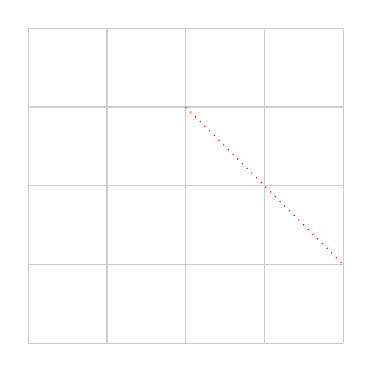
\begin{tikzpicture}
            \draw[step=1,color=gray!40] (-2,2) grid (2,-2);
            \path(0,1) coordinate(p1); %两种方式定义起止坐标
            \coordinate(p2) at (2,-1); 
            \draw[dotted,red] (p1) -- (p2); %使用 -- 表示虚线
        \end{tikzpicture}
    \end{center}
    \vspace{12pt}

    Task2:使用控制点绘制弧形曲线 \\
    \vspace{12pt}
    \begin{center}
        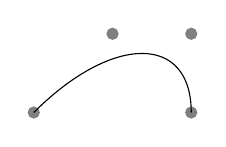
\begin{tikzpicture}
            \filldraw[gray] (0,0) circle (2pt) (1,1) circle (2pt) (2,1) circle (2pt) (2,0) circle (2pt); %描点
            \draw (0,0) .. controls (1,1) and (2,1) .. (2,0); %利用控制点绘制曲线
        \end{tikzpicture}
    \end{center}
    

    \vspace{12pt}
    %绘制圆形结点并指定位置标号
    \begin{center}
        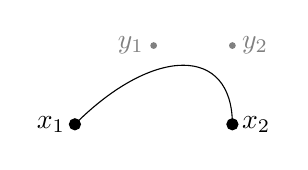
\begin{tikzpicture}
            \filldraw (0,0) circle [radius=2pt] node [left] {$ x _1$};
            \filldraw [gray] (1,1) circle [radius=1pt] node [left] {$ y _1$};
            \filldraw [gray] (2,1) circle [radius=1pt] node [right] {$ y_2$};
            \filldraw (2,0) circle [radius=2pt] node [right] {$ x _2$};
            \draw (0,0) .. controls (1,1) and (2,1) .. (2,0);
        \end{tikzpicture}
    \end{center}
    \vspace{12pt}

    \begin{center}
        \begin{tikzpicture}
            \filldraw[gray] (0,0) circle (1pt) (1,-2) circle (2pt) (2,3) circle (3pt) (4,-1) circle (4pt);
            \draw (0,0) .. controls (1,-2) and (2,3) .. (4,-1);
        \end{tikzpicture}
    \end{center}
    \vspace{12pt}

    \begin{center}
        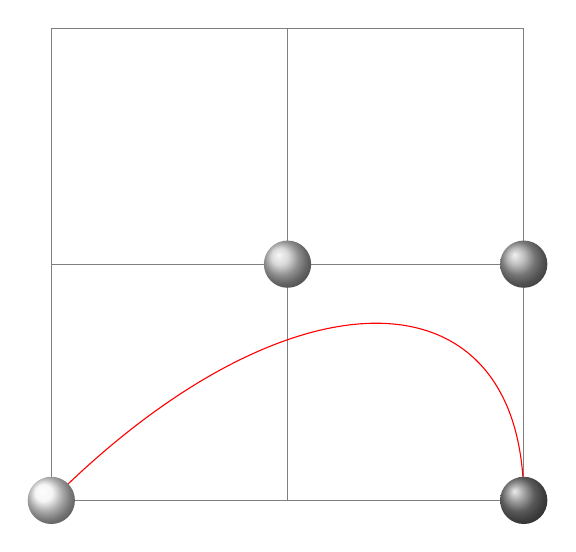
\begin{tikzpicture}[scale=3]  %设置缩放倍数
            \draw[help lines] (0,0) grid (2,2);  %实心网格线
            \draw[color=red] (0,0) .. controls (1,1) and (2,1) .. (2,0);  %绘制四大控制点
            \shade[ball color=gray!10] (0,0) circle (0.1);  %绘制不同灰度的球状阴影
            \shade[ball color=gray!40] (1,1) circle (0.1);
            \shade[ball color=gray!70] (2,1) circle (0.1);
            \shade[ball color=gray] (2,0) circle (0.1);
        \end{tikzpicture}
    \end{center}
    \vspace{12pt}

    \begin{center}
        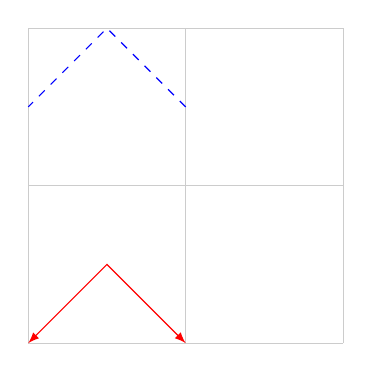
\begin{tikzpicture}[scale=1]
            \draw[step=2,color=gray!40] (-2,-2) grid (2,2);  
            \draw[latex-latex, red] (0,-2) -- ++(-1,1) -- ++(-1,-1); %使用++表示坐标随之更新
            \draw[dashed, blue] (0,1) -- +(-1,1) -- +(-2,0); %使用+表示坐标完全基于原点计算
        \end{tikzpicture}
    \end{center}
    \vspace{12pt}


    \begin{center}
        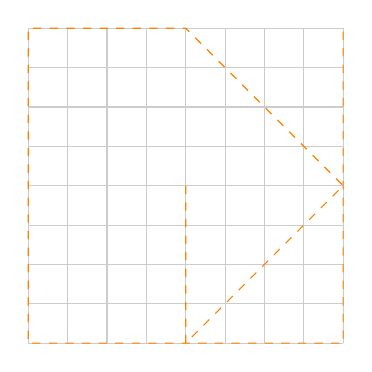
\begin{tikzpicture}[scale=1]
            \draw[step=0.5,color=gray!40] (-2,-2) grid (2,2);  
            \draw[dashed, orange] (0,0) -- ++(0,-2) -- ++(2,2) -- ++(-2,2) -- ++(-2,0) -- ++(0,-4) -- ++(4,0) -- ++(0,4);
        \end{tikzpicture}
    \end{center}
    \vspace{12pt}

    Task3:使用node绘制节点树图 \\
    \begin{center}
        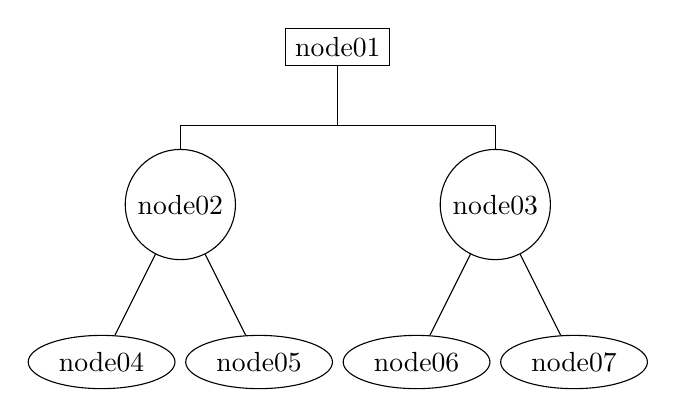
\begin{tikzpicture}[]
            \node (node01) at (0,2) [draw] {node01};
            \node (node02) at (-2,0) [shape=circle,draw] {node02};
            \node (node03) at (2,0) [shape=circle,draw] {node03};
            \draw (node cs:name=node01,anchor=south) |- (0,1);
            \draw (node02.north) |- (0,1) -| (node03.north);
            
            \node (node04) at (-3,-2) [shape=ellipse,draw] {node04};
            \node (node05) at (-1,-2) [shape=ellipse,draw] {node05};
            \node (node06) at (1,-2) [shape=ellipse,draw] {node06};
            \node (node07) at (3,-2) [shape=ellipse,draw] {node07};
            \draw (node02) -- (node04);
            \draw (node02) -- (node05);
            \draw (node03) -- (node06);
            \draw (node03) -- (node07);
        \end{tikzpicture}
    \end{center}
    \vspace{12pt}

    Task4:绘制两个路径的交点 \\
    \begin{center}
        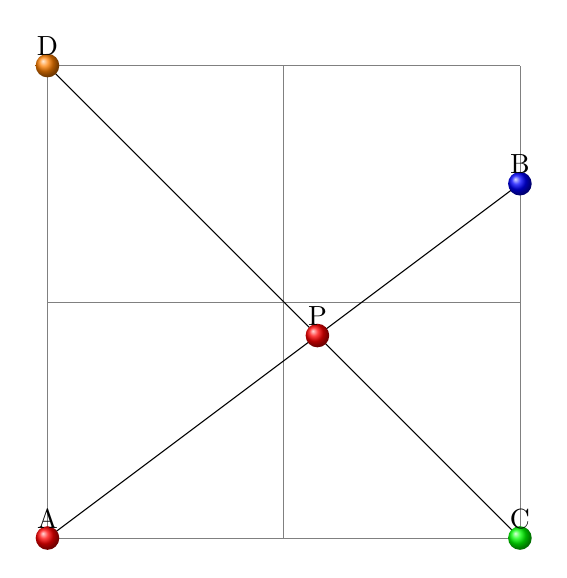
\begin{tikzpicture}[scale=3]
            \draw[help lines] (0,0) grid (2,2);
            \coordinate (A) at (0,0); %定义点的坐标
            \coordinate (B) at (2,1.5);
            \coordinate (C) at (2,0);
            \coordinate (D) at (0,2);
            \draw[name path=AB,below] (A) -- (B); %定义路径AB、CD
            \draw[name path=CD,below] (C) -- (D);
            \path[name intersections={of =AB and CD}] (intersection-1) coordinate (P);
            \shade[ball color=red](A) circle (0.05) node[above] {A}; %定义球形阴影
            \shade[ball color=blue](B) circle (0.05) node[above] {B};
            \shade[ball color=green](C) circle (0.05) node[above] {C};
            \shade[ball color=orange](D) circle (0.05) node[above] {D};
            \shade[ball color=red](P) circle (0.05) node[above] {P};
            \end{tikzpicture}
    \end{center}

    Task5:绘制坐标轴与一个半径为$\pi$的圆\\
    \begin{center}
        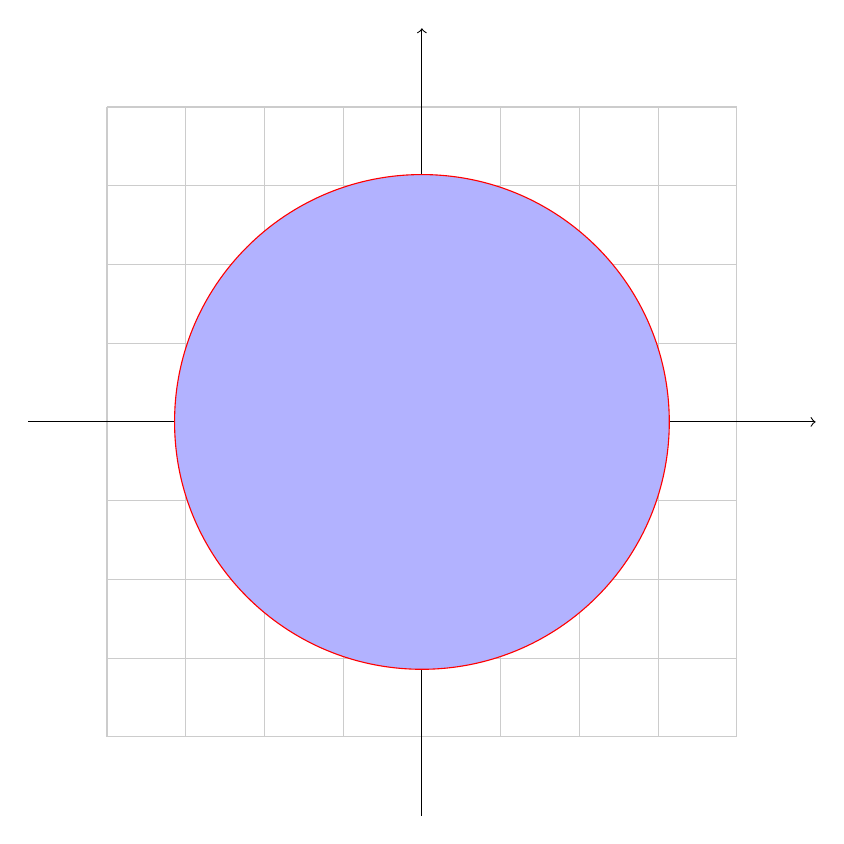
\begin{tikzpicture}
            \draw[step=1,color=gray!40] (-4,-4) grid(4,4);
            \draw[->] (-5,0) -- (5,0); %绘制坐标轴
            \draw[->] (0,-5) -- (0,5);
            \draw[red, fill = blue!30] (0,0) circle (3.1415);
        \end{tikzpicture}
    \end{center}
    \vspace{12pt}

    Task6:绘制椭圆与其焦点三角形 \\
    \begin{center}
        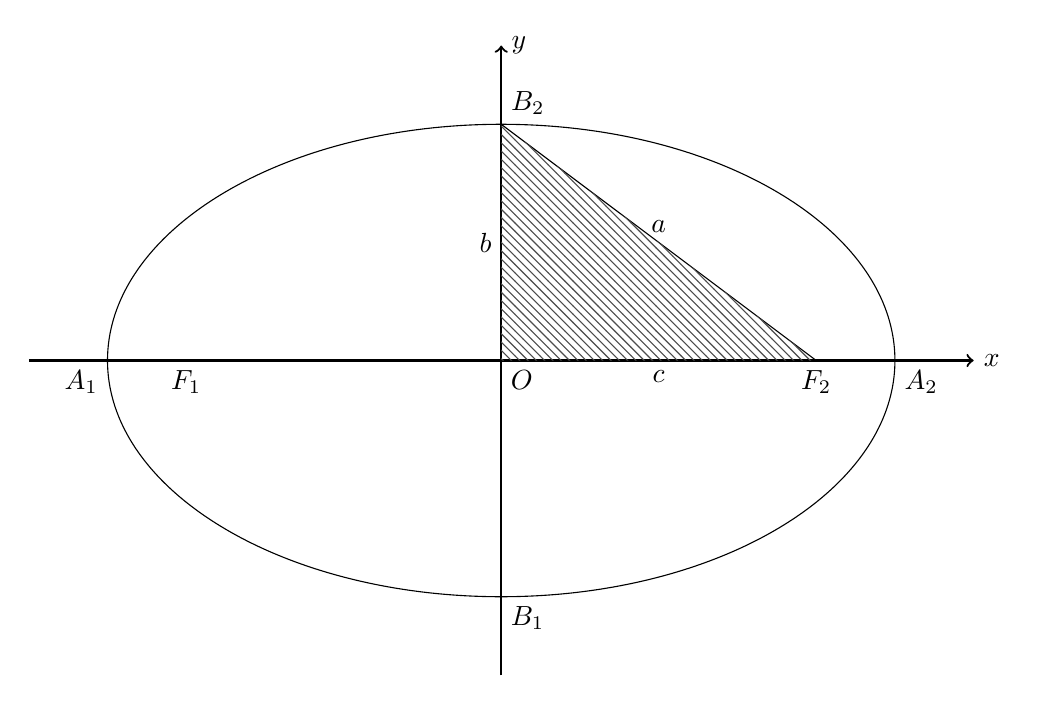
\begin{tikzpicture}
            \def\a{5}%长半轴
            \def\b{3}%短半轴
            \def\c{4}%焦半轴
            \path[name path=xaxis,thick,draw,->](-6,0)--(6,0) node[right] {$x$};
            \path[name path=yaxis,thick,draw,->](0,-4)--(0,4) node[above,right] {$y$};
            %x轴与y轴的交点
            \path [name intersections={of = xaxis and yaxis}];
            \coordinate[label=below right:$O$] (O) at (intersection-1); %在右下角设置坐标O文字
            \draw [name path = myellipse] (intersection-1) ellipse (\a cm and \b cm);%绘制椭圆路径
            \path [name intersections={of = xaxis and myellipse}];
            \coordinate[label=below right:$A_2$] (a2) at (intersection-1); %intersection的结果默认左2右1(合理猜测是按照逆时针方向从x正半轴开始计数 intersection-No.x.)
            \coordinate[label=below left:$A_1$] (a1) at (intersection-2); %给长轴交点标号
            \path [name intersections={of = yaxis and myellipse}];
            \coordinate[label=above right:$B_2$] (b2) at (intersection-1);
            \coordinate[label=below right:$B_1$] (b1) at (intersection-2);
            \coordinate[label=below :$F_1$] (f1) at (-\c,0); %绘制焦点位置
            \coordinate[label=below :$F_2$] (f2) at (\c,0);
            \draw (b2) -- (f2) node[midway,above] {$a$}; %绘制焦点三角形并填充阴影
            \draw (b2) --(O) node[midway,left] {$b$};
            \draw (O) --(f2) node[midway,below] {$c$};
            \fill [pattern =north west lines,pattern color = black!70](b2)--(O)--(f2)--cycle; %从左上到右下的斜线
        \end{tikzpicture}
    \end{center}
    \vspace{12pt}

    Task7:绘制三大圆锥曲线并练习scope环境的用法 \\
    \begin{center}
        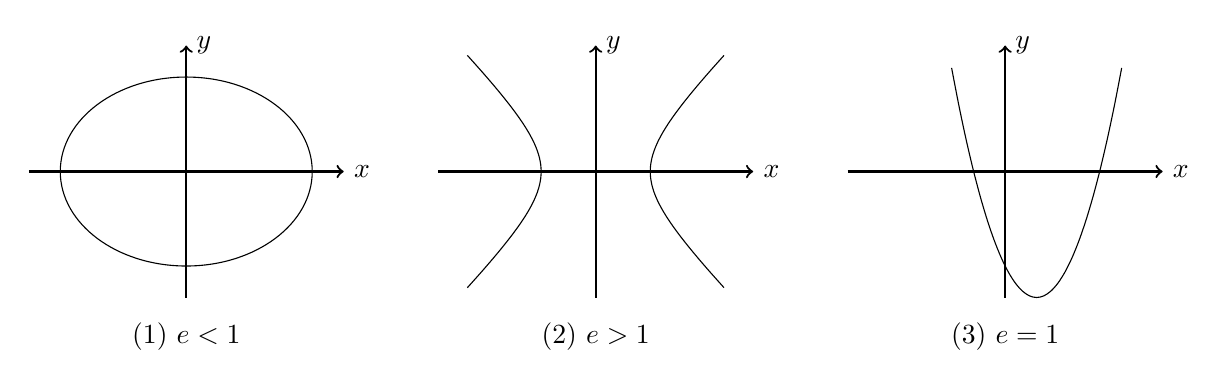
\begin{tikzpicture}[scale=0.4]
            % 椭圆
            \path[thick,draw,->](-5,0)--(5,0) node[right] {$x$};
            \path[thick,draw,->](0,-4)--(0,4) node[above,right] {$y$};
            \draw (0,0) ellipse (4 cm and 3 cm);
            \node[below] at (0,-4.5) {$(1)\ e<1$};
            
    
            \begin{scope}[xshift=13cm]
                \path[thick,draw,->](-5,0)--(5,0) node[right] {$x$};
                \path[thick,draw,->](0,-4)--(0,4) node[above,right] {$y$};
                %%利用双曲函数来表示双曲线方程
                \draw[domain=-1.5:1.5, smooth, variable=\x] plot ({1.732*cosh(\x)}, {1.732*sinh(\x)});
                \draw[domain=-1.5:1.5, smooth, variable=\x] plot ({-1.732*cosh(\x)}, {1.732*sinh(\x)});
                \node[below] at (0,-4.5) {$(2)\ e>1$}; 
            \end{scope}
    
            \begin{scope}[xshift=26cm]
                \path[thick,draw,->](-5,0)--(5,0) node[right] {$x$};
                \path[thick,draw,->](0,-4)--(0,4) node[above,right] {$y$};
                \draw[domain=-1.7:3.7, smooth, variable=\x] plot ({\x}, {\x*\x-2*\x-3});
                \node[below] at (0,-4.5) {$(3)\ e=1$}; 
            \end{scope}
          \end{tikzpicture}
    \end{center}
    \vspace{12pt}

    Task8:绘制圆状太极图案 \\
    \begin{center}
        
\begin{tikzpicture}[scale=0.8]
            \draw(0,0) circle(4cm); %画一个4cm的圆圈
            %把圆的右半边填黑
            \begin{scope}
                \clip(0,0) circle(4cm); %%裁剪区域,故后续的rectangle命令只作用于被裁剪过的圆形区域
                \fill[black] (0,-4) rectangle (4,4);
            \end{scope}
            %填黑八卦图左边的半圆
            \begin{scope}
                \clip(0,2) circle(2cm);
                \fill[black] (-4,0) rectangle (4,4);
            \end{scope}
            %填白八卦图右边的半圆
            \begin{scope}
                \clip(0,-2) circle(2cm);
                \fill[white] (-4,0) rectangle (4,-4);
            \end{scope}
            %把黑色部分的小圆圈填为白色
            \begin{scope}
                \clip(0,2) circle(0.5cm);
                \fill[white] (-4,0) rectangle (4,4);
            \end{scope}
            %绘制下面的白色圆圈
            \draw(0,-2) circle(0.5cm);
          \end{tikzpicture}
    \end{center}
    \vspace{12pt}

    Task9:绘制Gauss经典的圆内接正十七边形 \\
    \begin{center}
        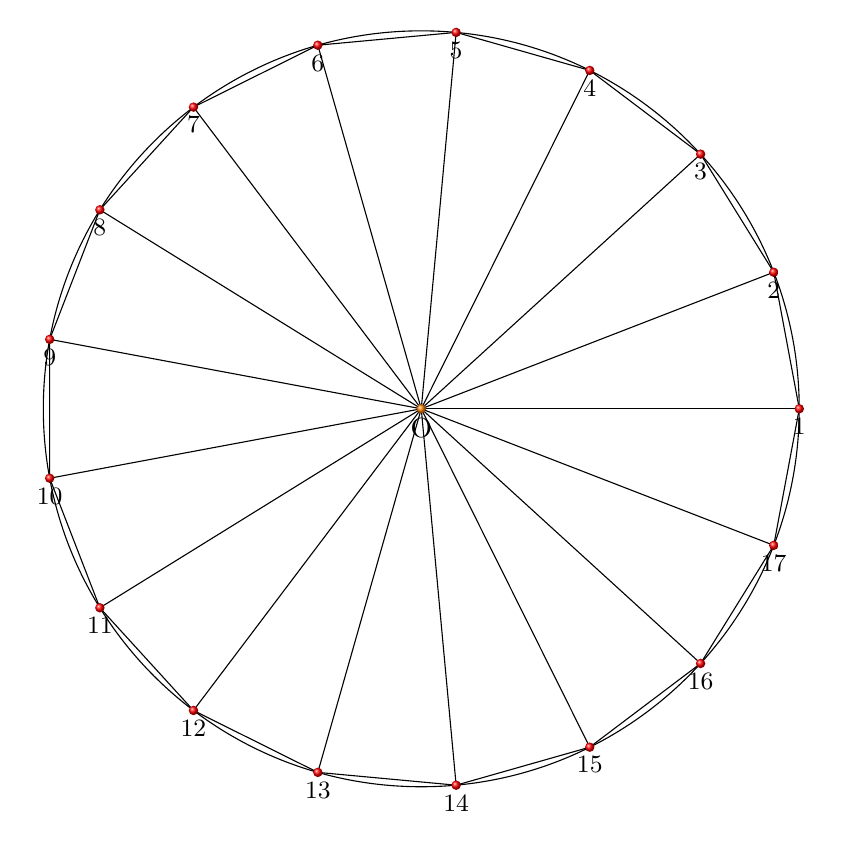
\begin{tikzpicture}[scale=1.2]
            \draw (0,0) circle(4);
            \coordinate (O) at (0,0);
            %%使用pgf的循环方法来画图
            \def\n{17}
            \pgfmathsetmacro{\i}{\n-1}
            \foreach \x in {0,...,\i}{ %从0~n-1进行循环画点\x
            \def\pointname{\x}
            \coordinate (\pointname) at ($(0,0)+(\x*360/\n:4cm)$);  %%第\x个点的极坐标写法为坐标为(0rad,0distance) \x*360/\n 为极角 而 :4cm意为半径
            \draw (O) -- (\x); %%绘制圆心的连线
            }
        \draw (0) \foreach \x in {0,...,\i} { -- (\x) } -- cycle; %整行绘图命令,包含x0~x16
        \shade[ball color=orange] (O) circle (0.05) node[below] {O};
        \foreach \x in {0,...,\i}{ 
            \def\pointname{\x}
            \pgfmathtruncatemacro{\ii}{\x+1} %需使用calc库进行计算,其中\pgfmathtruncatemacro保证计算结果为整数
            \shade[ball color=red] (\pointname) circle(0.05) node[below] {\small \ii};
        }
        \end{tikzpicture}
    \end{center}
    \vspace{12pt}


    Task10:使用help lines绘制花里胡哨网格图\\
    \begin{center}
        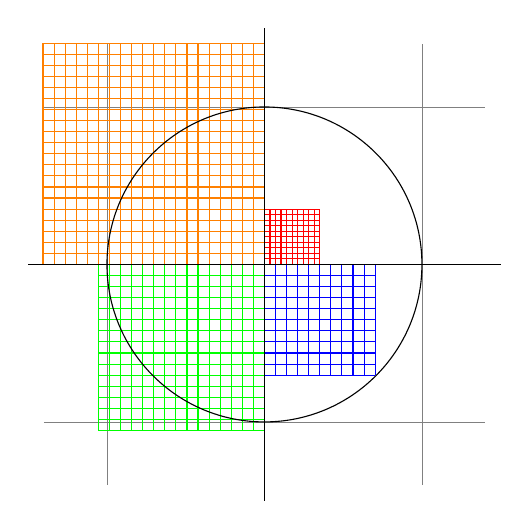
\begin{tikzpicture}[scale=2]
            \draw[help lines] (-1.4,-1.4) grid (1.4,1.4); %绘制背景大网格图
            \draw[step=1pt,color=red] (0,0) grid (10pt,10pt);
            \draw[step=2pt,color=blue] (0,0) grid (20pt,-20pt);
            \draw[step=2pt,color=green] (0,0) grid (-30pt,-30pt);
            \draw[step=2pt,color=orange] (0,0) grid (-40pt,40pt);
            \draw (-1.5,0) -- (1.5,0);
            \draw (0,-1.5) -- (0,1.5);
            \draw (0,0) circle (1cm);
        \end{tikzpicture}
    \end{center}
    \vspace{12pt}

    Task11:使用rounded corners选项绘制光滑线段图\\
    \begin{center}
        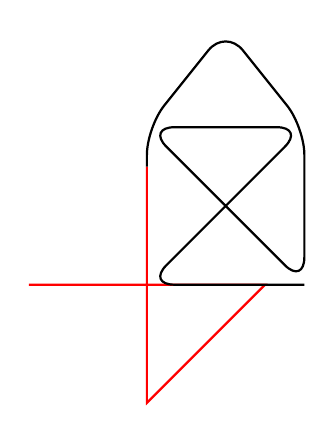
\begin{tikzpicture}
            %瞎画的一段曲线段~
            \draw[thick, color=red, ] (-1.5,0) -- (1.5,0) -- (0,-1.5) -- (0,1.5);
            \draw[thick, rounded corners=10pt] (0,1.5) -- (0,2) -- (1,3.25) --
            (2,2) -- (2,0) -- (0,2) -- (2,2) -- (0,0) -- (2,0);
            \end{tikzpicture}
    \end{center}
    \vspace{12pt}
    
    Task12:绘制花里胡哨的箭头\\
    \begin{center}
        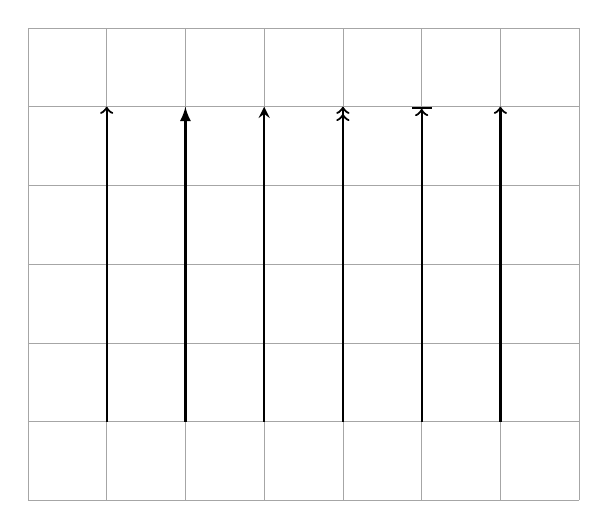
\begin{tikzpicture}
            \draw[help lines,color=gray!70] (-3,-3) grid (4,3);
            \draw[->,thick] (-2,-2) -- (-2,2);
            \draw[-latex,thick] (-1,-2) -- (-1,2);
            \draw[-stealth,thick] (0,-2) -- (0,2);
            \draw[->>,thick] (1,-2) -- (1,2);
            \draw[->|,thick] (2,-2) -- (2,2);
            \draw[-to,thick] (3,-2) -- (3,2);
        \end{tikzpicture}
    \end{center}
    \vspace{12pt}

    Task13:使用arc选项绘制圆弧\\
    \begin{center}
        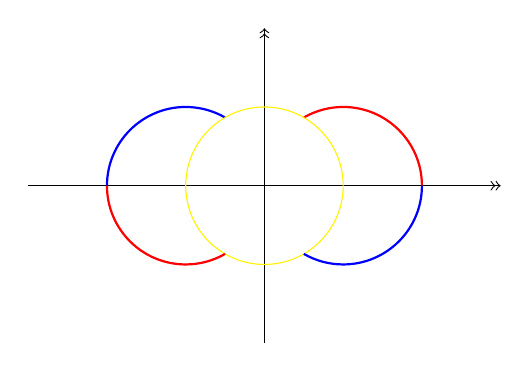
\begin{tikzpicture}
            \draw[->>] (-3,0) -- (3,0);
            \draw[->>] (0,-2) -- (0,2);
            \draw[thick,color=red] (2,0) arc (0:120:1cm);  %绘制半径为1cm,角度为[0,120°]的圆弧
            \draw[thick,color=blue] (-2,0) arc (180:60:1cm);
            \draw[color=yellow] (0,0) circle (1cm);
            \draw[thick,color=red] (-2,0) arc (180:300:1cm);
            \draw[thick,color=blue] (2,0) arc (360:240:1cm);  
        \end{tikzpicture}
    \end{center}
    \vspace{12pt}

    Task14:绘制正弦函数图像与其定义\\
    \begin{center}
        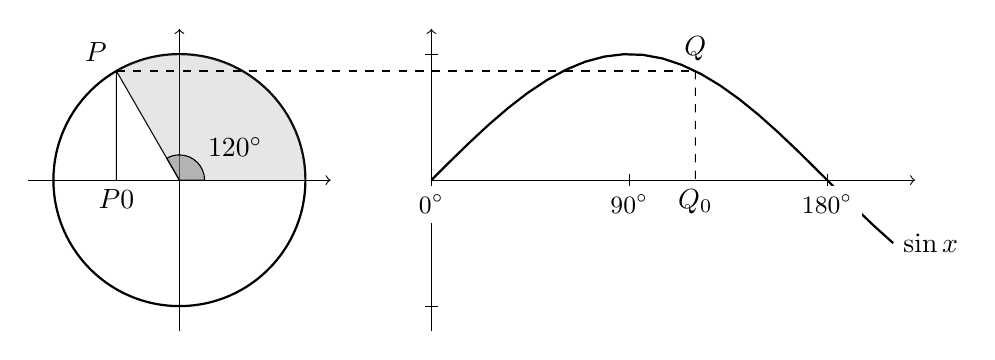
\begin{tikzpicture}[scale=1.6]
            \def\iangle{120}
            \begin{scope}[xshift=-2cm]  %位移2cm
                \draw[->] (-1.2,0) --(1.2,0);
                \draw[->] (0,-1.2) --(0,1.2);
                \draw[thick] (0,0) circle(1cm);
                \coordinate [label = \iangle:$P$] (P) at (\iangle:1);
                \coordinate [label = below:$P0$] (P0) at (P |-0,0);
                \draw (P)--(P0);
                \draw (0,0)--(P);
                \fill [fill = gray,fill opacity=0.2] (0,0)--(0:1) arc (0:\iangle:1) -- cycle; %两点+一段圆弧围成封闭图形
                \filldraw [fill = gray,fill opacity=0.5] (0,0)--(0:0.2) arc (0:\iangle:0.2) -- cycle; 
                \node [right] at (\iangle/2:0.3) {\ang{\iangle}}; %标识角度
            \end{scope}

            \draw[->] (0,0) -- ({rad(220)},0);
            \draw[->] (0,-1.2) -- (0,1.2);
            \draw [thick,domain=0:rad(210)] plot (\x,{sin(\x r)}) node [right] {$\sin x$}; %指定 sin\x的计算方式为弧度制
            
            \foreach \t in {0,90,180}{ %利用循环在x轴上标点,并用白色块覆盖
                \draw ({rad(\t)},-0.05)--({rad(\t)},0.05) ;
                \node [below, outer sep =2pt, font=\small, fill = white] at ({rad(\t)},0) {\ang
                {\t}};
            }
            \foreach \y in {-1,1}{  %利用循环在y轴上标点
                \draw (-0.05,\y) -- (0.05,\y);
            }
            \coordinate [label=above:{$Q$}] (Q) at ({rad(\iangle)},{sin(\iangle)}); %标识P、Q点
            \coordinate [label=below:{$Q_0$}] (Q0) at (Q |- 0,0);
            \draw[dashed] (Q)--(Q0);
            \draw[dashed] (P) --(Q);
        \end{tikzpicture}

        
    \end{center}


    Task15:设置样式绘制三角函数定义图\\
    \begin{center}
        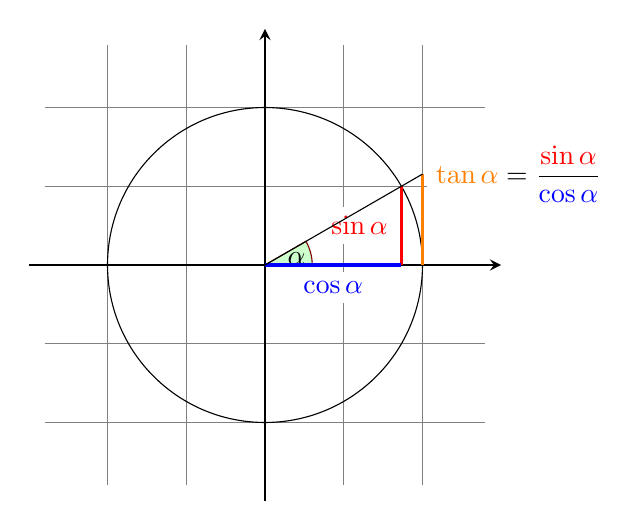
\begin{tikzpicture}[scale=2, >= stealth] %设置箭头均为stealth类型
            \draw[step=0.5cm,gray,very thin] (-1.4,-1.4) grid (1.4,1.4);
            \filldraw[fill=green!20!white,draw=red!50!black] (0,0) -- (3mm,0mm) arc [start angle=0, end angle=30, radius=3mm] -- cycle; %标识角度
            \draw (2mm, 0.4mm) node {$\alpha$};
            \draw[->,thick] (-1.5,0) -- (1.5,0) coordinate (x axis);
            \draw[->,thick] (0,-1.5) -- (0,1.5) coordinate (y axis);
            \draw (0,0) circle [radius=1cm];
            
            \draw[red,very thick] (30:1cm) -- node[left=1pt, fill=white] {$\sin \alpha$} +(0,-0.5);
            %%绘制红色的sin\alpha直线  从(30°,1cm)出发,向下移动-0.5个单位
            \draw [blue,very thick] (30:1cm) ++(0,-0.5) -- node[below=2pt,fill=white] {$\cos \alpha$} (0,0);
            %%绘制蓝色的cos\alpha直线  从(30°,1cm)出发,先向下移动-0.5个单位,此后用蓝色直线标记向左回到(0,0)
            \draw [orange,very thick] (1,0) -- (1,{tan(30)}) node[right=1pt,fill=white]{$\displaystyle \tan \alpha \color{black}=\frac{{\color{red}\sin \alpha }}{\color{blue}\cos \alpha}$};
            %%绘制橙色的tan\alpha直线  从(1,0)出发,移动到点(1,{tan(30)})并添加公式
            \draw (0,0) -- (1,{tan(30)}); %绘制斜边
        \end{tikzpicture}
    \end{center}
    \vspace{12pt}

    Task16:基于样式设置进行绘图\\
    \begin{itemize}
        \item 全局设置: 在导言区加入设置 \verb|\tikzset{style_name./style={options}}|.
        \item 局部设置: 在\verb |\tikzpicture| 环境内使用\verb | [style_name/.style={options}] |.
        \item 分层样式全局设置: \verb |\tikzset{style_name1/.style={style_name2, options}} |.
        \item 分层样式局部设置: \verb |[style_name1/.style={style_name2, options}]|.
        \item 分层样式与参数局部设置: \verb |[style_name/.style={option1s},style_name/.default={option2s}]|.
    \end{itemize}
    \begin{center}
        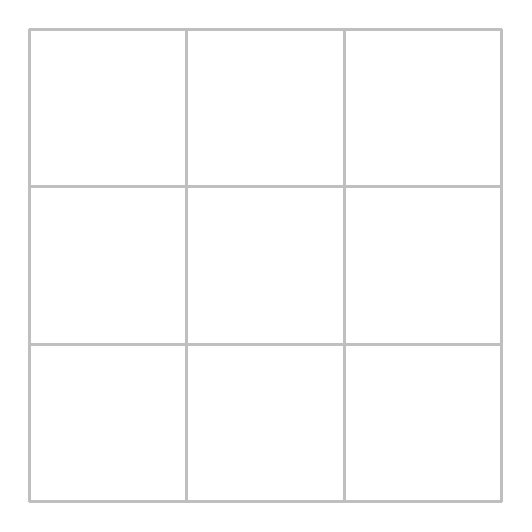
\begin{tikzpicture}
            [red_thick_lines/.style={color=gray!50,very thick}];
            \draw[step=2cm, red_thick_lines] (0,0) grid (6,6);
        \end{tikzpicture}\\
        \vspace{30pt}
        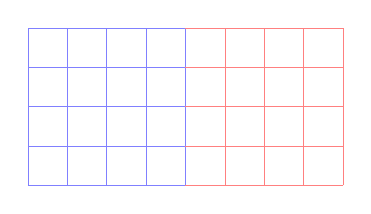
\begin{tikzpicture}
            [para_color/.style={help lines,color=#1!50}, para_color/.default=blue]
            \draw[step=0.5cm, para_color] (0,0) grid (2,2);
            \draw[step=0.5cm, para_color=red] (2,0) grid (4,2);
        \end{tikzpicture}\\
        \vspace{30pt}
        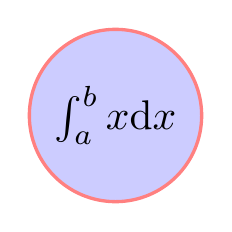
\begin{tikzpicture}
            [LNode/.style={circle, draw=red!50, fill=blue!20, very thick, minimum size=10mm,scale=1.5}]
            \node[LNode] (n1) at (0, 0){$\int_a^b x \mathrm{d}x$};
        \end{tikzpicture}
    \end{center}
    \vspace{12pt}

    Task17:基于pgfplots宏包进行绘图\\
    \begin{center}
        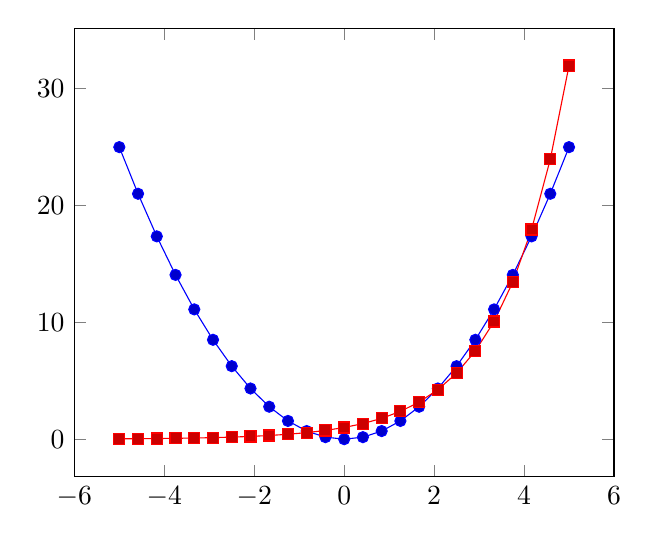
\begin{tikzpicture}
            \begin{axis}
                \addplot {x^2};
                \addplot {2^x};
            \end{axis}
        \end{tikzpicture}\\
        \vspace{30pt}
        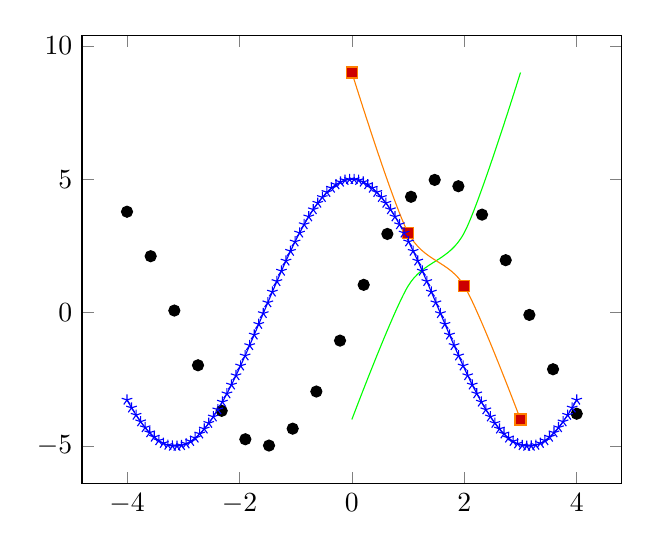
\begin{tikzpicture}
            \begin{axis}
                %使用smooth指定光滑 使用domain指定域 使用samples指定抽样本数 使用only marks指定只用标记
                \addplot[color=green,smooth] coordinates {(0,-4) (1,1) (2,3) (3,9)};
                \addplot+[color=orange,smooth] coordinates {(3,-4) (2,1) (1,3) (0,9)};
                \addplot[domain=-4:4, samples=20, only marks] {5*sin(deg(x))}; %使用deg(x)转换为弧度制
                \addplot+[domain=-4:4, samples=100, color=blue,smooth] {5*cos(deg(x))};
            \end{axis}
        \end{tikzpicture}\\
        \vspace{30pt}
        %view设置角度,trig format plots指定弧度制 title设置题目标题
        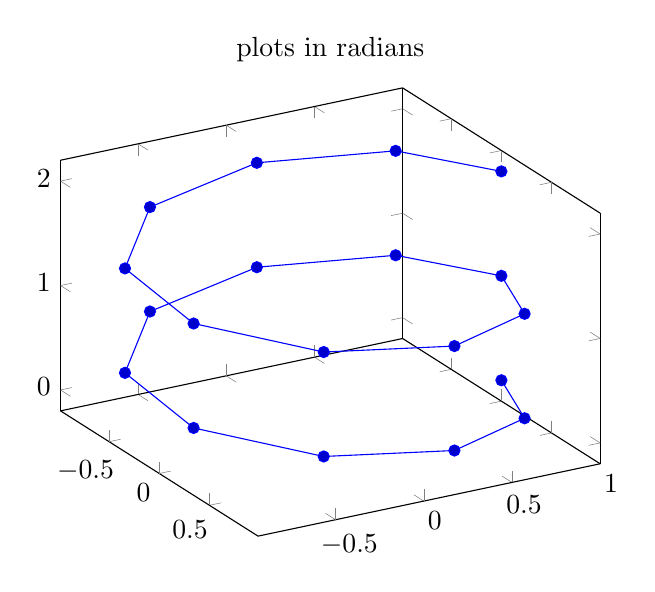
\begin{tikzpicture}
            \begin{axis}[view={60}{30},trig format plots=rad,title=plots in radians]
                \addplot3+ [domain=0:4*pi,samples=19,samples y=1]({sin(x)},{cos(x)},{2*x/(4*pi)});
                %设定\addplot3命令的x,y,z坐标
            \end{axis}
        \end{tikzpicture}\\
        \vspace{30pt}
        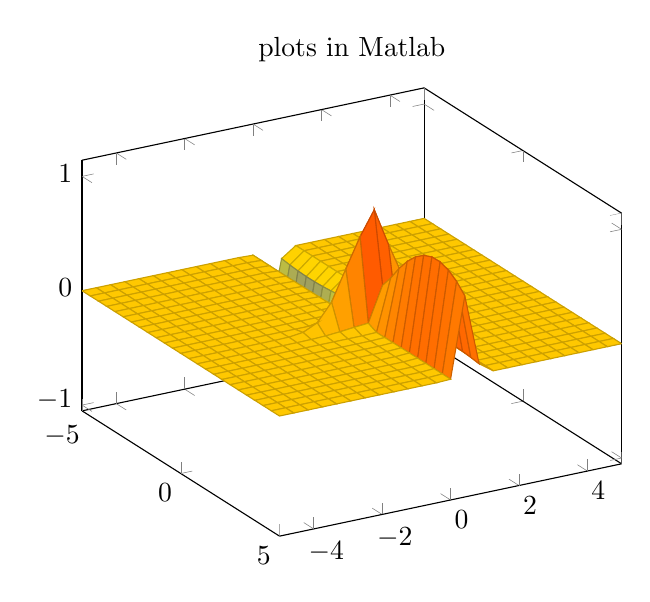
\begin{tikzpicture}
            \begin{axis}[view={60}{30},title=plots in Matlab]
                \addplot3[surf]{sin(8*pi*x)*exp(-20*(y-0.5)^2)+exp(-(x-0.5)^2*30-(y-0.25)^2-(x-0.5)*(y-0.25))};
            \end{axis}
        \end{tikzpicture}
    \end{center}
    \vspace{12pt}


    Task18:pgfplots宏包绘图实战演练\\
    \begin{center}
        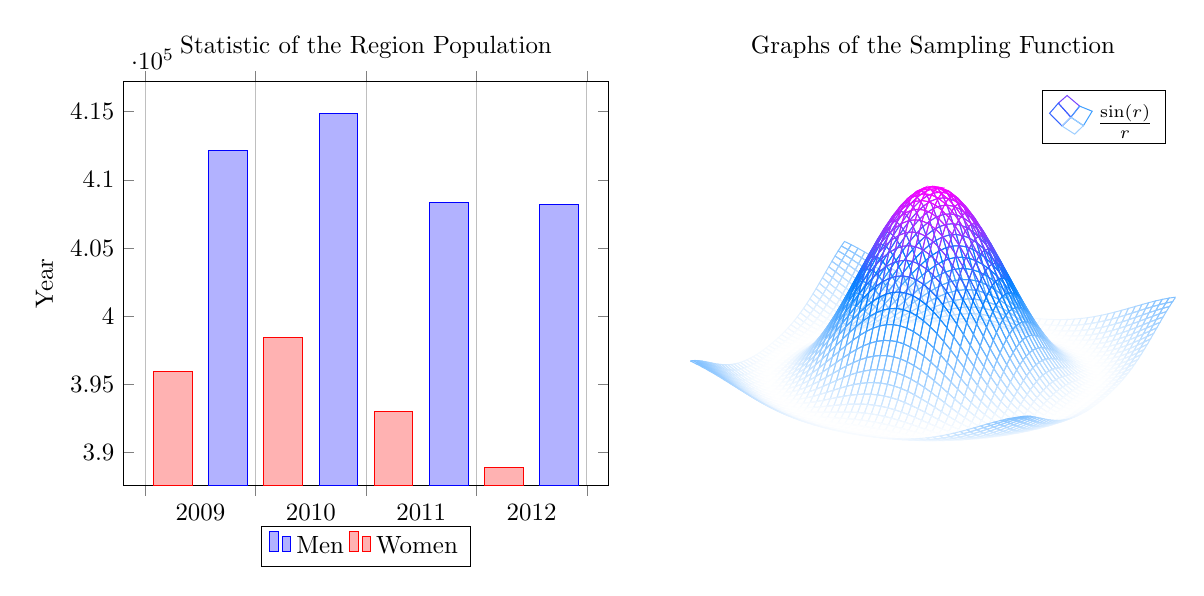
\begin{tikzpicture}[scale=0.9]
            \begin{axis}[
                x tick label style={/pgf/number format/1000 sep=},
                %%设置年份的千位分隔符为空
                ylabel=Year,
                ybar interval=0.7,
                enlargelimits=0.05,
                legend style={at={(0.5,-0.1)},anchor=north,legend columns=-1},
                title= Statistic of the Region Population,
                ]
                \addplot coordinates {(2012,408184) (2011,408348) (2010,414870) (2009,412156) (2008,415 838)};
                \addplot coordinates {(2012,388950) (2011,393007) (2010,398449) (2009,395972) (2008,398866)}; %引入坐标值
                \legend{Men,Women}
            \end{axis}
            \begin{scope}[xshift=8cm]
                \begin{axis}[
                        title=Graphs of the Sampling Function,
                        hide axis,
                        colormap/cool,
                    ]
                    \addplot3[
                        mesh,
                        samples=50,
                        domain=-5:5,
                    ]{sin(deg(sqrt(x^2+y^2)))/sqrt(x^2+y^2)};
                    \addlegendentry{$\frac{\sin(r)}{r}$} %添加legend图例
                \end{axis}
            \end{scope}
            
        \end{tikzpicture}\\
        
    \end{center}
    \vspace{12pt}

    

\end{document}

